%==============================================================================
% Closing the Variance Gap: Bochner PINN for Lévy-Driven SPDEs
% Hubert Lipski
%
% Version 4: incorporates all experimental findings from the Heston-V
% diagnosis campaign (subgrid overfit, randomized subgrid fix, cumulant
% matching for kurtosis, Lévy intensity tau-sweep).
%
% Key changes from v3:
%  - Abstract: Heston-V "structural failure" replaced by diagnosis + fix
%  - §1.3 Contributions: three new bullets (subgrid overfit, cumulant, Lévy tau)
%  - §2 Method: new §2.6 randomized spectral sub-grid
%  - §3.4 Theory Remark: reframed from "structural failure" to "initial diagnosis"
%  - §5 Results: new §5.5 Heston-V diagnosis with 2×4 ablation table
%  - §6 Discussion: "Heston variance channel: diagnosed and fixed" replaces
%   "a documented failure"
%  - §7 Conclusion: updated
%  - Appendix A: Lévy intensity threshold sweep (negative result)
%==============================================================================

\documentclass[10pt]{elsarticle}

\usepackage[utf8]{inputenc}
\usepackage[T1]{fontenc}
\usepackage{amsmath, amsthm, amssymb}
\usepackage{booktabs}
\usepackage{multirow}
\usepackage{siunitx}
\usepackage{graphicx}
\usepackage{hyperref}
\usepackage[disable]{microtype}
\usepackage{tikz}
\usetikzlibrary{positioning, arrows.meta, shapes.geometric}

\graphicspath{{figures/}}

\newtheorem{remark}{Remark}
\newtheorem{proposition}{Proposition}
\newtheorem{lemma}{Lemma}
\newtheorem{corollary}{Corollary}

\journal{Journal of Computational Physics}

\begin{document}

\begin{frontmatter}

\title{Closing the Variance Gap: Bochner PINN for Physics-Informed Learning on Stationary Random Fields}

\author{Hubert Lipski}

\begin{abstract}
Standard PINNs trained on stochastic PDEs converge to the conditional
mean of the solution law; MSE training provides no distributional
signal.
We introduce \emph{Bochner PINN}, augmenting the standard loss with
log-spatial PSD, log-temporal PSD, and variance ratio terms evaluated
against a finite-difference reference on a randomised spectral
sub-grid.
For stationary \emph{Gaussian} random fields with separable covariance,
combining Bochner's theorem with the Gelbrich--Givens--Shortt formula
and a kernel-smoothed periodogram estimator yields a single-realisation
$W_2$ bound
\(W_2 \le C_1\sqrt{\varepsilon} + C_2 N_s^{-\beta_{\rm sr}} +
C_3\sqrt{\delta}\) with $\beta_{\rm sr} = s_x/(2(2s_x+d))$
and explicit constants. For \emph{L\'evy}-driven fields the same
bound holds for the Gaussian projection of the law (second-order
structure).
We validate on L\'evy-driven SPDEs: variance ratio rises from
\(0.19\) to \(0.83\) on a hierarchical Variance-Gamma SPDE, the same
loss closes the gap on four of five FNO benchmarks.
\end{abstract}

\begin{keyword}
physics-informed neural networks \sep
stochastic partial differential equations \sep
stationary random fields \sep
spectral methods \sep
distributional convergence \sep
L\'evy processes
\end{keyword}

\end{frontmatter}

%==============================================================================
\section{Introduction}
\label{sec:intro}

\subsection{Motivation}
\label{subsec:motivation}

Many physical and financial systems are governed by stochastic PDEs
whose solutions are random fields rather than deterministic functions.
Accurate surrogate models for such systems must reproduce the
\emph{probability law} of the solution, not merely its mean, since
downstream quantities such as tail risk, variance, and higher moments
depend critically on the full distribution.
Physics-informed neural networks (PINNs) are natural candidates for
efficient surrogate modelling: their inference cost is \(O(|\theta|)\),
independent of spatial resolution and dimension once trained, making
them attractive for real-time applications where classical solvers are
prohibitively expensive.
The problem addressed here is that standard PINN training systematically
fails to recover the law: the MSE loss contains no distributional
signal, so the network converges to the conditional mean of the random
field and loses variance, tail structure, and spectral content.

The failure is especially acute for SPDEs driven by L\'evy processes,
which are the primary validation setting of this paper.
L\'evy-driven dynamics arise across financial risk management,
statistical mechanics, and plasma physics (non-local heat transport in
Tokamak reactors), and they capture jump discontinuities and
heavy-tailed distributions essential for extreme climatic events and
biological foraging under the L\'evy Flight Foraging Hypothesis.
The non-local fractional Laplacian operator compounds the difficulty:
FD discretisations produce dense matrices (\(O(N^{2d})\) storage,
prohibitive at \(N=32\), \(d=4\)) and MC methods converge at
\(O(n^{-1/2})\), rendering both impractical for real-time use.
The distributional failure of vanilla PINNs therefore closes off the
one computationally efficient path.

\subsection{The Problem}
\label{subsec:problem}

The core difficulty is that standard PINN losses constrain neither the
probability law of the random field nor its frequency content across
realisations. The NTK eigenvalue spectrum governs which frequency
components the network learns; low-frequency eigenvalues dominate
standard training, so the network learns the general shape of the
solution and discards the high-frequency structure that encodes
variance and tail behaviour. This spectral-bias account is correct for
deterministic PDEs but understates the stochastic problem: the
relevant learning target is the \emph{probability law} of the random
field, and MSE on collocation points provides no signal about it
whatsoever.

For the Lévy-driven SPDEs studied here, the problem is compounded by
the non-local fractional Laplacian: FD discretisation produces dense
matrices, and the PINN must impose a non-local integral operator
through a local smooth neural-net structure. But this is a secondary
difficulty. The primary failure, the network converging to the
conditional mean of the law, occurs even when the operator is local
and the noise is mild. It is a structural property of MSE training on
stochastic problems, not a consequence of heavy tails or non-locality.

\subsection{Contribution}
\label{subsec:contribution}

We propose the \emph{Bochner PINN}, a drop-in modification to the
standard PINN that augments the conventional loss with three
distributional regularisers evaluated on a spectral sub-grid against a
finite-difference reference: spatial power spectral density, temporal
power spectral density, and variance ratio. The construction is
theoretically motivated by Bochner's theorem, which guarantees that
for stationary Gaussian random fields with separable space-time
covariance, matching spectral marginals recovers the second-order law.

The central claim of this paper is that for stochastic PDEs the
correct learning objective is convergence of the predictor's
probability law to the reference law, and that Bochner's theorem
identifies the spectral density as the natural matching quantity.
The contributions are:

\begin{itemize}
\item \textbf{Distributional convergence theorem (Gaussian forcing).}
We prove that matching the kernel-smoothed log-power spectral density
on a Sobolev-regular spectral sub-grid implies Wasserstein-2
convergence of laws for stationary Gaussian random fields with
separable covariance, with explicit constants and an explicit rate:
\(W_2 \leq C_1\sqrt{\varepsilon} + C_2 N_s^{-\beta_{\rm sr}}
+ C_3\sqrt{\delta}\) with $\beta_{\rm sr} = s_x/(2(2s_x+d))$ valid
for a single realisation of $u_\theta$ and $u_{\rm FD}$ under
$\alpha$-mixing of the reference field (Proposition~\ref{thm:main}).
The proof extends the Mishra--Molinaro framework with three new
lemmas (log-to-linear spectral control, kernel-smoothed
periodogram consistency, Plancherel--Gelbrich bound) and is the
first single-realisation distributional convergence result for
Bochner PINN training. We also establish partial results for the
L\'evy regime: a Gaussian-projection bound that controls only the
second-order structure
(Proposition~\ref{thm:levy-ext}); full-law and higher-cumulant extensions are given in the extended version.

\item \textbf{Identification of the variance failure mode.} We quantify
vanilla PINN variance underestimation on L\'evy SPDEs across three
problem classes: a factor of \(\sim 5\times\) on the hierarchical
3-channel Fokker-Planck system, \(\sim 2\times\) on Burgers-VG, and a
complete variance collapse (\(\mathrm{vr} \approx 0\)) on the
Heston-VG price channel. This is a distributional failure, the
network converges to the conditional mean of the law, not a
frequency-resolution failure of the kind studied in the deterministic
spectral bias literature.

\item \textbf{Bochner PINN method.} A simple drop-in modification:
three distributional regularisers grounded in Bochner's theorem, with
no change to architecture, optimiser, or training data.

\item \textbf{Bayesian baseline.} A mean-field Bayes-by-Backprop PINN
trained at identical architectural parameters fails by 7--33\(\times\)
on log-spatial PSD MSE relative to the deterministic vanilla baseline,
demonstrating that variational uncertainty quantification over network
weights does not substitute for an explicit distributional loss.

\item \textbf{Per-component ablation.} A 5-variant \(\times\) 5-seed
ablation on Burgers-VG demonstrates that the three loss terms are
nearly orthogonal: each targets its own metric, single-term
variants are unstable, and only the full combination achieves
uniform improvement (Section~\ref{subsec:ablation}).

\item \textbf{Bochner FNO.} The same loss applied to a
Fourier Neural Operator surrogate closes the variance gap on four
of five problems (a 2D Navier--Stokes vorticity benchmark and a
Black--Scholes 2D L\'evy benchmark are added as out-of-class
controls), with the largest gain a sixteen-fold closure on
Heston-VG (Section~\ref{sec:spectral-fno}). The construction is
therefore architecture-agnostic.

\item \textbf{Empirical validation.} Across three synthetic L\'evy-SPDE
classes, consistent variance-gap closure: \(0.19 \to 0.83\) on the
most-driven hierarchical channel, \(0.50 \to 0.93\) on Burgers-VG,
and \(0.14 \to 0.93\) on the Heston volatility channel after
randomised sub-grid training.

\item \textbf{Honest characterisation.} An explicit account of where
Bochner PINN provides marginal benefit (the \(y\)-channel seed
outlier in the hierarchical SPDE, the S-channel kurtosis of Heston-VG)
and the structural reason in each case.
\end{itemize}

\section{Method}
\label{sec:method}

\begin{figure}[t]
 \centering
 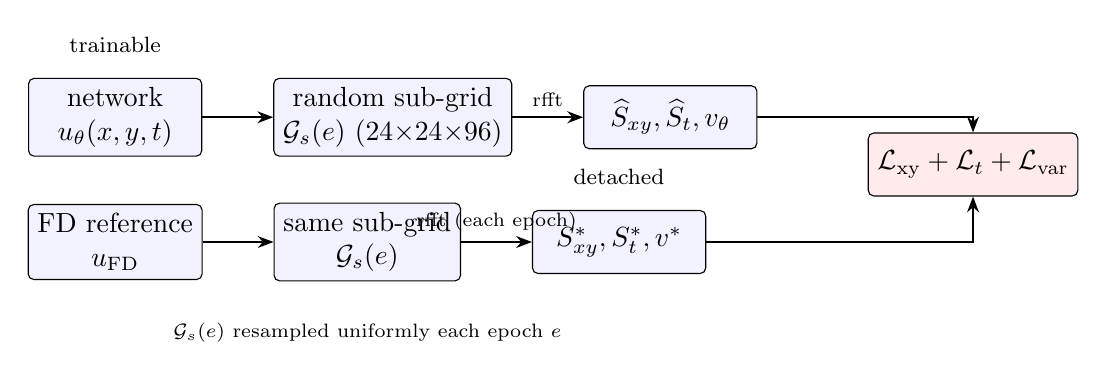
\begin{tikzpicture}[
   box/.style={draw, rounded corners=2pt, align=center,
         minimum height=8mm, minimum width=22mm, fill=blue!5},
   lossbox/.style={draw, rounded corners=2pt, align=center,
           minimum height=8mm, minimum width=24mm, fill=red!8},
   arr/.style={-{Stealth[length=2mm]}, thick},
   node distance=6mm and 9mm,
  ]
  \node[box] (uth) {network\\$u_\theta(x,y,t)$};
  \node[box, below=of uth] (uFD) {FD reference\\$u_{\mathrm{FD}}$};
  \node[box, right=of uth] (subth) {random sub-grid\\$\mathcal{G}_s(e)$ ($24{\times}24{\times}96$)};
  \node[box, right=of uFD] (subFD) {same sub-grid\\$\mathcal{G}_s(e)$};

  \node[box, right=of subth] (psdth) {$\widehat S_{xy}, \widehat S_t, v_\theta$};
  \node[box, right=of subFD] (psdFD) {$S^*_{xy}, S^*_t, v^*$};

  \node[lossbox, right=14mm of psdth, yshift=-6mm] (loss)
    {$\mathcal{L}_{\mathrm{xy}} + \mathcal{L}_{t} + \mathcal{L}_{\mathrm{var}}$};

  \draw[arr] (uth)  -- (subth);
  \draw[arr] (uFD)  -- (subFD);
  \draw[arr] (subth) -- node[above, font=\scriptsize]{rfft} (psdth);
  \draw[arr] (subFD) -- node[above, font=\scriptsize]{rfft (each epoch)} (psdFD);
  \draw[arr] (psdth) -| (loss);
  \draw[arr] (psdFD) -| (loss);

  \node[font=\footnotesize, above=2mm of uth] {trainable};
  \node[font=\footnotesize, above=2mm of psdFD] {detached};

  \node[below=4mm of subFD, font=\scriptsize, align=center]
    {$\mathcal{G}_s(e)$ resampled uniformly each epoch $e$};
 \end{tikzpicture}
 \caption{Bochner PINN: at each epoch $e$ the network $u_\theta$ and
 the FD reference $u_{\mathrm{FD}}$ are both evaluated on a sub-grid
 $\mathcal{G}_s(e)$ drawn uniformly at random from the full FD grid.
 Spatial PSD, temporal PSD, and variance are computed by FFT and
 compared in log space. The random re-sampling at each epoch prevents
 sub-grid overfit (Section~\ref{subsec:rand-subgrid}).}
 \label{fig:method-schematic}
\end{figure}

\subsection{What goes wrong with the standard PINN}

Train a vanilla PINN on a L\'evy-driven SPDE and inspect three
diagnostics on a held-out grid:
\begin{enumerate}
\item Pointwise relative \(L^2\) error: \(\approx 0.3\) (acceptable).
\item Variance ratio
\(\mathrm{Var}\,u_\theta / \mathrm{Var}\,u_{\mathrm{FD}}\):
\(\approx 0.2\)--\(0.5\).
\item Power spectrum \(|\mathcal F u_\theta|^2\) vs
\(|\mathcal F u_{\mathrm{FD}}|^2\): high modes are missing by 2--4
decades.
\end{enumerate}
The network is averaging across the noise realisation rather than
reproducing it. Pointwise loss is insensitive to high-frequency
content because high-frequency error and high-frequency signal
cancel almost exactly under MSE. Any sample-path-style use of
\(u_\theta\) (extracting tail statistics, computing exit times,
valuing a path-dependent option) fails. We close this gap by
adding three loss terms that directly penalise the missing
structure.

\subsection{Three terms, three diagnostics}
\label{subsec:losses}

Compute the FD reference once and extract three statistics on a
sub-grid \(\mathcal{G}_s\) of resolution \(24 \times 24 \times 96\):
the spatial power spectrum \(S^*_{xy}(k)\), the temporal power
spectrum \(S^*_t(k)\), and the total variance \(v^*\). At every epoch
we evaluate \(u_\theta\) on \(\mathcal{G}_s\) and form the matching
statistics \(S_{xy}, S_t, v_\theta\). The new loss components are
\begin{align}
\mathcal{L}_{\mathrm{xy}} &=
\overline{\bigl(\log_{10}S_{xy} - \log_{10}S^*_{xy}\bigr)^2}, &
\mathcal{L}_{\mathrm{t}} &=
\overline{\bigl(\log_{10}S_t - \log_{10}S^*_t\bigr)^2}, \notag\\
\mathcal{L}_{\mathrm{var}} &= \bigl((v_\theta - v^*)/v^*\bigr)^2.
\label{eq:losses}
\end{align}
\(\mathcal{L}_{\mathrm{xy}}\) and \(\mathcal{L}_{\mathrm{t}}\)
correct \emph{shape}; \(\mathcal{L}_{\mathrm{var}}\) corrects
\emph{scale}. The spatial PSD is computed symmetrically along both
spatial axes,
\begin{equation}
\widehat S_{xy}(f) = \tfrac12
\Bigl(\overline{|\mathcal F_x f|^2}_{y,t}
+ \overline{|\mathcal F_y f|^2}_{x,t}\Bigr),
\end{equation}
so anisotropic features that align with one axis do not bias the
metric. The temporal PSD
\(\widehat S_t(f) = \overline{|\mathcal F_t f|^2}_{x,y}\) is
averaged over space.

\subsection{Why log, why MSE, why a sub-grid}

\textbf{Log scale.} Power spectra span 4--6 orders of magnitude on
L\'evy problems. A linear loss would care only about the lowest few
wavenumbers, exactly the regime the vanilla PINN already gets
right. Working in \(\log_{10}\) assigns equal weight to each decade
and makes the high-mode discrepancy visible to the optimiser.

\textbf{MSE in log space.} Equivalent to a symmetric Bregman
divergence between the two empirical spectral measures up to an
additive constant, and \emph{asymptotically} equivalent to a
Whittle-type negative log-likelihood for the periodogram via the
Gumbel limit of the log-periodogram
\cite{Whittle1953,Dahlhaus1996,Brillinger1981} (they share the same
population minimiser \(\mu = \mu_{u_{\mathrm{FD}}}\) and the same
\(\mathcal O(\log^{-2} N)\) score-function geometry near it, but
differ at finite sample size by the per-mode Gumbel-variance residual
analysed in the extended version).
The minimiser is \(u_{\mathrm{FD}}\) itself: the loss is consistent
in the sense that no other matching measure achieves zero (modulo
the realisation-noise residual discussed in
the extended version).

\textbf{Sub-grid.} The FFTs cost
\(O(n_x n_y n_t (\log n_x + \log n_y + \log n_t))\) per epoch.
Using the full FD grid would dominate the wall time; the
\(24 \times 24 \times 96\) sub-grid keeps spectral evaluation under
5\,\% of total compute while preserving all wavenumbers up to the
Nyquist frequency of \(\mathcal{G}_s\), which empirically captures
the regime where the variance gap is generated.

\subsection{Total objective and architecture}
\label{subsec:total-objective}

The Bochner PINN minimises
\begin{equation}
\mathcal{L}(\theta) =
\underbrace{\mathcal L_{\mathrm{PDE}}
+ \lambda_{\mathrm{ic}} \mathcal L_{\mathrm{IC}}
+ \lambda_{\mathrm{bc}} \mathcal L_{\mathrm{BC}}
+ \lambda_{\mathrm d} \mathcal L_{\mathrm{data}}}_{\text{physics}}
+ \underbrace{\lambda_{\mathrm{xy}} \mathcal L_{\mathrm{xy}}
+ \lambda_{\mathrm t} \mathcal L_{\mathrm t}
+ \lambda_{\mathrm v} \mathcal L_{\mathrm{var}}}_{\text{spectral}}.
\label{eq:total-loss}
\end{equation}
The physics block is the standard PINN objective:
\(\mathcal L_{\mathrm{PDE}}\) is the squared collocation residual
under the SPDE on a fresh batch of 4096 uniform samples each epoch,
with the L\'evy-Gamma jump and white-noise terms supplied by spline
interpolation of the precomputed driver fields;
\(\mathcal L_{\mathrm{IC}}, \mathcal L_{\mathrm{BC}}\) are MSE
penalties on initial and boundary data; \(\mathcal L_{\mathrm{data}}\)
is the MSE against \(u_{\mathrm{FD}}\) at random grid points.

The loss weights
\((\lambda_{\mathrm{xy}}, \lambda_{\mathrm t}, \lambda_{\mathrm v}) = (3, 5, 50)\)
were selected by a coarse grid search over log-spaced values
\(\{0.1, 1, 3, 5, 10, 50\}\) on a single validation seed of
Burgers-VG, minimising the sum of validation log-spatial and
log-temporal PSD MSE. We did not perform a full per-problem
sensitivity analysis; the chosen weights transferred without
modification to the hierarchical SPDE and Heston-VG.

The network \(u_\theta\) is a four-block residual MLP of width 96
(128 for jump-driven problems) with \(\tanh\) activations, preceded
by a frozen random-Fourier-feature embedding
\(\phi(v) = [\sin(2\pi B v), \cos(2\pi B v)]\) with
\(B \in \mathbb R^{(d+1)\times m}\),
\(B_{ij} \sim \mathcal N(0, s^2)\). We use \(m=64, s=3\) for jump
problems and \(m=48, s=2\) otherwise. Optimisation is Adam with
cosine-annealed learning rate \(10^{-3} \to 10^{-6}\) and gradient
clipping \(\|g\|_2 \le 5\). A 1000-epoch warmup deactivates
\(\mathcal L_{\mathrm{PDE}}\) to let IC and data fit stabilise; the
spectral losses are active from epoch 1.

\subsection{Randomised spectral sub-grid}
\label{subsec:rand-subgrid}

\emph{Why a fixed sub-grid fails.} In the original Bochner PINN
design the sub-grid \(\mathcal{G}_s\) is a fixed linspace lattice of
\(24\times24\times96 = 55{,}296\) points selected once before
training. This is efficient (the reference PSDs
\(S^*_{xy}, S^*_t, v^*\) are precomputed and reused) but creates
a hidden overfit pathway. Because the network sees exactly the same
points each epoch, gradient descent can satisfy
\(\mathcal{L}_{\mathrm{spec}}\) by memorising those \(55{,}296\)
grid values while interpolating near zero elsewhere. On the full
\(48\times48\times512 \approx 1.2 \times 10^6\) grid the variance
ratio then collapses, even though the sub-grid spectral loss reads
near zero (the extended version).

\emph{Fix: epoch-wise random resampling.} At the start of each
training epoch we draw a fresh sub-grid of size
\(24\times24\times96\) by sampling indices uniformly without
replacement along each axis independently:
\begin{equation}
 \mathcal{G}_s(e) =
 \bigl(\pi_x^{(e)}, \pi_y^{(e)}, \pi_t^{(e)}\bigr),
 \quad
 \pi_x^{(e)} \sim \mathrm{Uniform}\{0,\ldots,N_x{-}1\}_{24},
 \label{eq:rand-subgrid}
\end{equation}
and likewise for \(y, t\). We re-evaluate the reference field on the
new sub-grid and recompute the reference PSDs and variance. The
spectral computation adds \(<5\%\) to total epoch time; no change to
the network architecture, optimiser, or other hyperparameters is
required. The resampling forces the network to match the spectral
statistics at \emph{every} subset of the domain, ruling out the
memorisation shortcut.

\subsection{Hyperparameters}
\label{subsec:hyper}

\begin{table}[h]
\centering
\caption{Hyperparameters used by all methods. Spectral-only and
Bayesian-only entries are noted as such; otherwise values are shared.}
\label{tab:hyper}
\begin{tabular}{l l l}
\toprule
symbol & value & role \\
\midrule
\(L,\,H\)          & 4,\, 96--128 & depth, width \\
\(m,\,s\)          & 48--64,\, 2--3 & Fourier feature count, scale \\
\(n_x,\,n_y,\,n_t\)     & 24,\, 24,\, 96 & spectral sub-grid resolution \\
sub-grid sampling       & random (each epoch) & prevents sub-grid overfit \\
\(\lambda_{\mathrm{ic}}\)  & 50 & IC weight \\
\(\lambda_{\mathrm{bc}}\)  & 10 & BC weight \\
\(\lambda_{\mathrm d}\)   & 5 & data weight \\
\(\lambda_{\mathrm{xy}}\)  & 3 (spectral only) & log-spatial PSD weight \\
\(\lambda_{\mathrm{t}}\)   & 5 (spectral only) & log-temporal PSD weight \\
\(\lambda_{\mathrm{v}}\)   & 50 (spectral only) & variance weight \\
\(\lambda_{\mathrm{kurt}}\) & 10 (cumulant mode) & fourth-cumulant weight \\
\(\lambda_{\mathrm{KL}}\)  & \(1/(B_c+B_d)\) (Bayesian only) & KL weight \\
prior \(\sigma\) (Bayesian) & 1.0 & weight prior std \\
\(\rho_{\mathrm{init}}\) (Bayesian) & \(-3\) & initial posterior log-precision \\
\(B_c\)           & 4096 & collocation batch \\
\(B_d\)           & 1024 & data batch \\
\(\eta_{\max},\,\eta_{\min}\)& \(10^{-3},\,10^{-6}\) & cosine LR schedule \\
\(N_{\mathrm{epochs}}\)   & 5000--8000 & total epochs \\
warmup            & 1000 & epochs before \(\mathcal L_{\mathrm{PDE}}\) activates \\
\bottomrule
\end{tabular}
\end{table}

\section{Why the spectral loss matches the law: motivation and scope}
\label{sec:theory}

This section motivates the loss introduced in Section~\ref{sec:method}
and identifies the class of fields on which it is provably the right
object. Section~\ref{subsec:convergence} establishes a quantitative
convergence rate (Proposition~\ref{thm:main}) for the class on which the
proof is rigorous --- stationary \emph{Gaussian} random fields with
separable covariance, trained with the kernel-smoothed periodogram
loss --- extending the Mishra--Molinaro
framework~\cite{MishraMolinaro2022,DeRyckMishra2022} to spectral
training losses. The extended version states partial
results for the L\'evy-driven case and is honest about what is
\emph{not} proved there: the rigorous bound on the full law of
non-Gaussian solutions requires either an additive $O(\sqrt{\nu})$
correction (the full-law extension) that vanishes only in the
small-jump limit, or a different proof technique
(characteristic-function distance, Stein--Malliavin) outside the
scope of this paper. The Variance-Gamma experiments in
Section~\ref{sec:results} are therefore best read as empirical
evidence that the spectral loss recovers second-order structure for
L\'evy drivers as well, with the rigorous full-law bound a
follow-up direction.

\subsection{Spectral measures determine second-order structure}

Let \(u : \Omega \times [0, T] \to \mathbb R\) be a mean-zero,
weakly stationary random field. Its covariance kernel
\(K_u(\tau, h) = \mathbb E[u(t,x)\,u(t+\tau, x+h)]\) admits the
Bochner representation~\cite[Thm.~9.18]{RudinRCA}
\begin{equation}
K_u(\tau, h) = \int_{\mathbb R^d \times \mathbb R}
e^{i(\omega \tau + k \cdot h)}\,\mathrm d\mu_u(\omega, k),
\qquad \mu_u\text{ positive and finite},
\label{eq:bochner}
\end{equation}
where \(\mu_u\) is the spectral measure of \(u\). Two reductions
are relevant for our discrete loss: the spatial marginal
\(\mu^{\mathrm{xy}}_u(k) = \int \mathrm d \mu_u(\omega, k)\) and
the temporal marginal
\(\mu^t_u(\omega) = \int \mathrm d \mu_u(\omega, k)\), which are
matched (in their discrete-sample analogues \(S^*_{xy}\),
\(S^*_t\)) by the Bochner PINN.

\paragraph{Separability assumption.}
Matching \(\mu^{\mathrm{xy}}_u\) and \(\mu^t_u\) separately
recovers the joint spectral measure \(\mu_u\) only when the
covariance kernel factorises, \(K_u(\tau, h) = K_x(h)\, K_t(\tau)\),
equivalently \(\mathrm d\mu_u(\omega, k) = \mathrm d\mu^{\mathrm{xy}}_u(k)\,
\mathrm d\mu^t_u(\omega)\). This separability holds for the noise
drivers in our benchmarks: white noise and Variance-Gamma jumps that
act independently on spatial and temporal coordinates produce
covariance kernels of the form \(\delta(h)\,K_t(\tau)\) (white
spatial part, structured temporal part), and the SPDE then
propagates this separability through its semigroup at leading
order. We adopt the separability assumption throughout.

For \emph{Gaussian} stationary fields under separability,
\(\mu_u\) determines the law completely: two such fields with
equal spectral measures are equal in distribution. The spectral
matching loss
\(\mathcal L_{\mathrm{xy}} + \mathcal L_t + \mathcal L_{\mathrm{var}}\)
therefore controls the law on this class.

For non-Gaussian L\'evy-driven fields, \(\mu_u\) determines only
the \emph{second-order structure}. Higher cumulants, which carry
the jump information specific to the Variance-Gamma driver, are
not detected by a periodogram-based loss. Closing this remaining
gap requires explicit cumulant matching, which we pursue in
the extended version.

\begin{remark}[Scope of the spectral loss]
\label{rem:scope}
Under the separability assumption, a zero of the spectral loss
characterises the law of the predictor on stationary Gaussian fields
(Bochner). Beyond identifiability, Proposition~\ref{thm:main} below
provides a quantitative convergence rate: the Wasserstein-2 distance
decomposes into a training-error term \(C_1\sqrt{\varepsilon}\), a
sub-grid quadrature term \(C_2 N_s^{-\beta_{\rm sr}}\), and a PDE-residual
term \(C_3\sqrt{\delta}\), with explicit constants. On stationary
L\'evy fields the same bound holds for the Gaussian projection of the
law (Proposition~\ref{thm:levy-ext}); higher cumulants are not controlled
and require a separate penalty (the extended version).
\end{remark}

\subsection{Quantitative convergence rate}
\label{subsec:convergence}

We now state the formal convergence rate. The rigorous main theorem
(Proposition~\ref{thm:main}) applies to stationary Gaussian random fields
under a kernel-smoothed version of the spectral loss; partial results
for L\'evy-driven fields are stated in
the extended version with frank discussion of the
remaining gaps.

\subsubsection{Assumptions}

The rigorous main theorem (Proposition~\ref{thm:main}) is stated under
six standing assumptions (A1)--(A6); (A5) Gaussianity is essential.
The L\'evy partial results in the extended version drop
(A5) at the cost of bounding only the Gaussian projection
(Proposition~\ref{thm:levy-ext}) or adding an $O(\sqrt{J})$ term
(the full-law extension, requiring (A7) $L^2$ jump control).
Assumptions (A8)--(A9) are required only for the conditional
results in Appendix~S1.

\begin{description}
\item[(A1) Stationarity and separability.] Both \(u_\theta\) and
\(u_{\mathrm{FD}}\) are centred, weakly stationary (after periodic
extension or sufficiently far from boundaries) with separable
covariance \(K(\tau, h) = K_x(h)\,K_t(\tau)\), equivalently
\(\mathrm d\mu(\omega, k) = \mathrm d\mu^{\mathrm{xy}}(k)\,
\mathrm d\mu^t(\omega)\).

\item[(A2) Sobolev regularity of spectra.]
\(\mu^{\mathrm{xy}} \in H^{s_x}(\widehat\Omega)\) and
\(\mu^t \in H^{s_t}(\widehat{[0,T]})\) with \(s_x > d/2\) and
\(s_t > 1/2\). This guarantees pointwise bounds and the \(L^2\)
FFT-quadrature error rate used in Lemma~S1.2 of the supplementary material.
For Variance-Gamma drivers \(s_x = s_t = 1\).

\item[(A3) Non-degeneracy.] There exist
\(0 < \mu_{\min} \le \mu_{\max} < \infty\) such that
\(\mu_{\min} \le \mu^{\mathrm{xy}}(k)\,\mu^t(\omega) \le \mu_{\max}\)
uniformly on the sub-grid frequency set
\(\widehat{\mathcal G}_s \subset \mathbb R^{d+1}\).

\item[(A4) Training tolerance.] At the end of training,
\begin{equation}
\mathcal L_{\mathrm{xy}}(u_\theta) + \mathcal L_t(u_\theta)
+ \mathcal L_{\mathrm{var}}(u_\theta) \le \varepsilon, \qquad
\mathcal L_{\mathrm{PDE}}(u_\theta)
+ \lambda_{\mathrm{ic}}\mathcal L_{\mathrm{IC}}(u_\theta)
+ \lambda_{\mathrm{bc}}\mathcal L_{\mathrm{BC}}(u_\theta)
\le \delta,
\label{eq:tolerance}
\end{equation}
for some \(0 < \varepsilon, \delta < \infty\), checked post hoc.

\item[(A5) Gaussianity (spectral leg only).] Both \(u_\theta\) and
\(u_{\mathrm{FD}}\) are centred Gaussian random fields on
\(\Omega \times [0,T]\). This hypothesis is required only for the
spectral path of the proof (Lemma~S1.5 of the supplementary material); the
PDE-residual path (Lemma~S1.6 of the supplementary material) holds without it.
Proposition~\ref{thm:levy-ext} below drops (A5) at the cost of
bounding the Gaussian projection only.

\item[(A6) Mixing condition (single-realisation consistency).]
\(u\) is \(\alpha\)-mixing with algebraic rate
\(\alpha(r) \le C_\alpha r^{-\gamma}\) for some \(\gamma > d+1\).
Variance-Gamma processes have independent increments, so
\(\alpha(r) = 0\) for all sufficiently large separations; the SPDE
solution inherits exponential spatial mixing from the Green's
function decay of the underlying parabolic operator~\cite{ContTankov2003}.
Assumption~(A6) is required for the main theorem's
single-realisation rate (Proposition~\ref{thm:main}), which controls
the kernel-smoothed periodogram on one sample path; without (A6)
only the expected-value bound of Lemma~S1.2 of the supplementary material is
available.

\item[(A7) L\'evy--It\^o decomposition with $L^2$ jump control.]
Both $u_\theta$ and $u_{\mathrm{FD}}$ admit L\'evy--It\^o decompositions
$u=u^G+u^J$ where $u^G$ is the Gaussian component and $u^J$ is the
pure-jump component~\cite{ContTankov2003}.
Assume
\[
\max\!\left(\mathbb{E}\|u_\theta^J\|^2_{L^2(\Omega\times[0,T])},\;
\mathbb{E}\|u_{\mathrm{FD}}^J\|^2_{L^2(\Omega\times[0,T])}\right)\le J
\]
for some finite $J\ge 0$ depending on the L\'evy parameters.
For Variance-Gamma drivers with kurtosis parameter $\nu$, $J=O(\nu)$
as $\nu\to 0$.
Assumption~(A7) is required only for
the full-law extension and is not used elsewhere.

\item[(A8) Finite pointwise cumulants.]
For each $(x,t)\in\Omega\times[0,T]$, the marginal law
$\mathcal{L}(u(x,t))$ has finite cumulants of order $m\le m_0$ for
some $m_0\ge 3$, with $|\kappa_m(u(x,t))|\le\bar\kappa_m<\infty$.
For Lévy-driven SPDEs, cumulants of $u(x,t)$ are bounded by
the $L^m$ norm of the Green's function times the corresponding driver
cumulants via the stochastic Fubini theorem.
Required only for the Berry--Esseen result.

\item[(A9) NTK lazy-training regime.]
The Bochner PINN is a two-layer network with $m$ neurons trained by
gradient flow. In the lazy-training regime the NTK Gram matrix $K$
with entries $K_{ij}=\nabla_\theta f(x_i)\cdot\nabla_\theta f(x_j)$
remains approximately constant throughout training, with minimum
eigenvalue $\lambda_{\min}(K)>0$.
Required only for Conjecture~S1.1 of the supplementary material.
\end{description}

Assumption (A1) is the scope identified above.
Assumption (A2) is satisfied by the VG drivers with
\(s_x = s_t = 1\). Assumption (A3) is restrictive: realistic
spectral measures decay polynomially in \(|k|\), so \(\mu_{\min}\)
is positive only after restriction to a finite frequency window;
the constants \(C_1, C_2\) of Proposition~\ref{thm:main} scale as
\(\mu_{\min}^{-1/2}\) and therefore degrade on that window's
high-frequency edge. Assumption (A4) is the endpoint of any
gradient-based training run.

\subsubsection{Main theorem}

The rigorous result uses the \emph{kernel-smoothed} periodogram
$\widehat S^{\mathrm{xy}}_h(u)(k) = \int \kappa_{h_N}(k-k')\,
\widehat S^{\mathrm{xy}}_{\mathcal G_s}(u)(k')\,dk'$ with bandwidth
$h_N^\star = N_s^{-1/(2s_x+d)}$ as the spectral loss target
(Lemma~S1.4 of the supplementary material in the supplementary material).
The smoothing is what makes the periodogram a consistent
single-realisation spectral estimator under (A6); without it the
raw periodogram has $\Theta(1)$ variance per Fourier mode that
does not vanish as $N_s \to \infty$, leaving a non-trivial residual
between the training loss and the true spectral $L^2$ distance.

\begin{proposition}[Single-realisation convergence rate of the
kernel-smoothed Bochner PINN]
\label{thm:main}
Under (A1)--(A6), with the spectral loss in (A4) evaluated against
the kernel-smoothed periodogram at the minimax-optimal bandwidth
$h_N^\star = N_s^{-1/(2s_x+d)}$, the Wasserstein-2 distance between
the laws of the Bochner PINN predictor and the FD reference satisfies
\begin{equation}
W_2\bigl(\mathcal L(u_\theta),\,\mathcal L(u_{\mathrm{FD}})\bigr)
\;\le\; C_1\sqrt{\varepsilon}
\;+\; C_2\,N_s^{-\beta_{\rm sr}}
\;+\; C_3\sqrt{\delta},
\label{eq:main-bound}
\end{equation}
with single-realisation exponent
\begin{equation}
\beta_{\rm sr} = \frac{s_x}{2\,(2 s_x + d)}
\;\le\;
\tfrac{1}{2}\min\!\bigl(s_x/d,\,s_t\bigr) =: \beta_{\rm bias},
\end{equation}
and constants
\(C_1 = \mu_{\max}\,\ln 10\,(M_{xy}+M_t) / \sqrt{2\mu_{\min}}\),
\(C_2 = (C_{\rm bias}+C_{\rm var})^{1/2}/\sqrt{2\mu_{\min}}\),
\(C_3 = \sqrt{C_{\mathrm{MM}}}\), where
\(M_{xy} = \|\mu_{xy,\mathrm{FD}}\|_{L^2}\),
\(M_t = \|\mu_{t,\mathrm{FD}}\|_{L^2}\), and
\(C_{\rm bias},\,C_{\rm var},\,C_{\mathrm{MM}}\) are explicit constants
defined in Appendix~S1.
\end{proposition}
\begin{proposition}[Second-order convergence for stationary
L\'evy fields]\label{thm:levy-ext}
Under~(A1)--(A4) but with $u_\theta,u_{\mathrm{FD}}$ not necessarily
Gaussian, denote by $\Pi_2\mathcal L(u)$ the centred Gaussian measure
with the same covariance as $\mathcal L(u)$ (the Gaussian projection).
Then
\[
W_2\!\bigl(\Pi_2\mathcal L(u_\theta),\,
\Pi_2\mathcal L(u_{\mathrm{FD}})\bigr)
\;\le\; C_1\sqrt{\varepsilon} + C_2 N_s^{-\beta_{\rm sr}} + C_3\sqrt\delta.
\]
\end{proposition}
\section{Experimental setup}
\label{sec:setup}

\subsection{Benchmark problems}
\label{subsec:problems}

\paragraph{Hierarchical 2D SPDE.}
A three-channel system on \([0,1]^2 \times [0, T]\) with channels
\((z, y, p)\): \(z\) driven by Variance-Gamma jumps, \(y\) by
Gamma jumps and a positivity constraint, and \(p\) representing a
probability density with a normalisation constraint. Boundary
conditions are Neumann on \(z, y\) and Dirichlet (zero) on \(p\).

\paragraph{Burgers-VG.}
Two-dimensional Burgers equation with multiplicative
Variance-Gamma jump forcing,
\begin{equation}
\partial_t u + \tfrac12 \nabla \cdot (u^2 \hat e)
= \nu \Delta u + \sigma \xi(x, y, t)
+ \mathrm dJ_{\mathrm{VG}}(x, y, t),
\label{eq:burgersvg}
\end{equation}
on \([0,1]^2 \times [0, T]\), Neumann boundary conditions, smooth
initial data. Variance-Gamma parameters
\((\sigma_{\mathrm{VG}}, \nu_{\mathrm{VG}}, \theta_{\mathrm{VG}})\)
follow Madan--Carr--Chang~\cite{MadanCarrChang1998}.

\paragraph{Heston-VG.}
Two-channel system \((S, V)\) for log-price and instantaneous
variance, with VG jumps in the price equation, Heston dynamics for
\(V\), and the standard Cox--Ingersoll--Ross stationarity
condition \(2\kappa\theta > \sigma^2\). Calibrated to plausible
equity parameters. The stationary distribution of \(V\) is
Gamma\((\nu, s)\) with \(\kappa_4 = 27.3\); the log-price channel
\(S\) has reference excess kurtosis \(\kappa_4 = 1460.8\) arising
from the compound VG jumps.

\subsection{Reference solver}

For each problem and seed we generate one finite-difference
reference solution \(u_{\mathrm{FD}}\) on a uniform grid. Spatial
discretisation uses second-order central differences; time
integration uses explicit Euler--Maruyama for the diffusion part
and a compound-Poisson sampler with VG-distributed jump sizes for
the L\'evy part following Cont--Tankov~\cite{ContTankov2003}.
Resolutions are \(64\times 64 \times 512\) for the hierarchical
SPDE and Burgers-VG, and \(48\times 48 \times 512\) for
Heston-VG. The same realisation \((\xi, J_{\mathrm{VG}})\) is then
re-sampled by spline interpolation during PINN training, so that
the PDE residual is evaluated against the same driver field as
the reference, eliminating sampling variability between solver and
surrogate.

\subsection{Metrics}
\label{subsec:metrics}

Let \(u_\theta, u_{\mathrm{FD}}\) be the predictor and reference
fields and \(\widehat S(\cdot)\) denote either the spatial or
temporal periodogram. We report:
\begin{itemize}
\item \textbf{Variance ratio}\quad
\(\mathrm{vr} = \mathrm{Var}(u_\theta)/\mathrm{Var}(u_{\mathrm{FD}})\),
target 1.
\item \textbf{Log-spatial PSD MSE}\quad
\(\overline{(\log_{10}\widehat S_{xy}(u_\theta) -
\log_{10}\widehat S_{xy}(u_{\mathrm{FD}}))^2}\), target 0.063
(the Euler--Mascheroni floor, see Section~\ref{sec:theory}).
\item \textbf{Log-temporal PSD MSE}\quad analogous on
\(\widehat S_t\).
\item \textbf{Relative \(L^2\)}\quad
\(\|u_\theta - u_{\mathrm{FD}}\|_2 / \|u_{\mathrm{FD}}\|_2\).
\item \textbf{Excess kurtosis}\quad
\(\kappa_4(u_\theta)\) vs.\ \(\kappa_4(u_{\mathrm{FD}})\), reported
for the Heston channels where higher-order matching is investigated.
\end{itemize}

\subsection{Baselines}

\paragraph{Vanilla deterministic PINN.} Identical architecture and
optimiser to the Bochner PINN with the spectral terms turned off
(\(\lambda_{\mathrm{xy}} = \lambda_t = \lambda_{\mathrm v} = 0\)).
This isolates the loss as the only difference.

\paragraph{Bayesian PINN (mean-field Bayes-by-Backprop).}
Mean-field variational PINN following~\cite{YangMengKarniadakis2021},
implemented with Gaussian variational posteriors over weights
(reparameterisation trick), \(\mathcal N(0, 1)\) prior, and a
closed-form KL regulariser scaled by \(1/(B_c + B_d)\). Same
depth, width, Fourier embedding, optimiser, and epoch budget as
the Bochner PINN. At evaluation we draw \(N = 64\) posterior
samples and report the metrics on the posterior mean, with the
posterior standard deviation noted as the epistemic uncertainty
estimate.

\subsection{Seeds and compute}

Random seeds are \(\{1,\ldots,8\}\) for the hierarchical SPDE,
\(\{0,\ldots,7\}\) for Burgers-VG, and \(\{0,\ldots,2\}\) for
Heston-VG. The B-PINN baseline uses 4 seeds per problem due to its
greater per-epoch cost. All Heston-VG diagnosis runs use 3 training
seeds evaluated against 5 validation seeds each (15 evaluations per
(subgrid, mode) cell of the 2\(\times\)4 ablation). All runs use a
single NVIDIA RTX-class GPU in fp32.

%==============================================================================
\section{Results}
\label{sec:results}

\subsection{Variance gap closure}
\label{subsec:gap}

\begin{figure}[t]
 \centering
 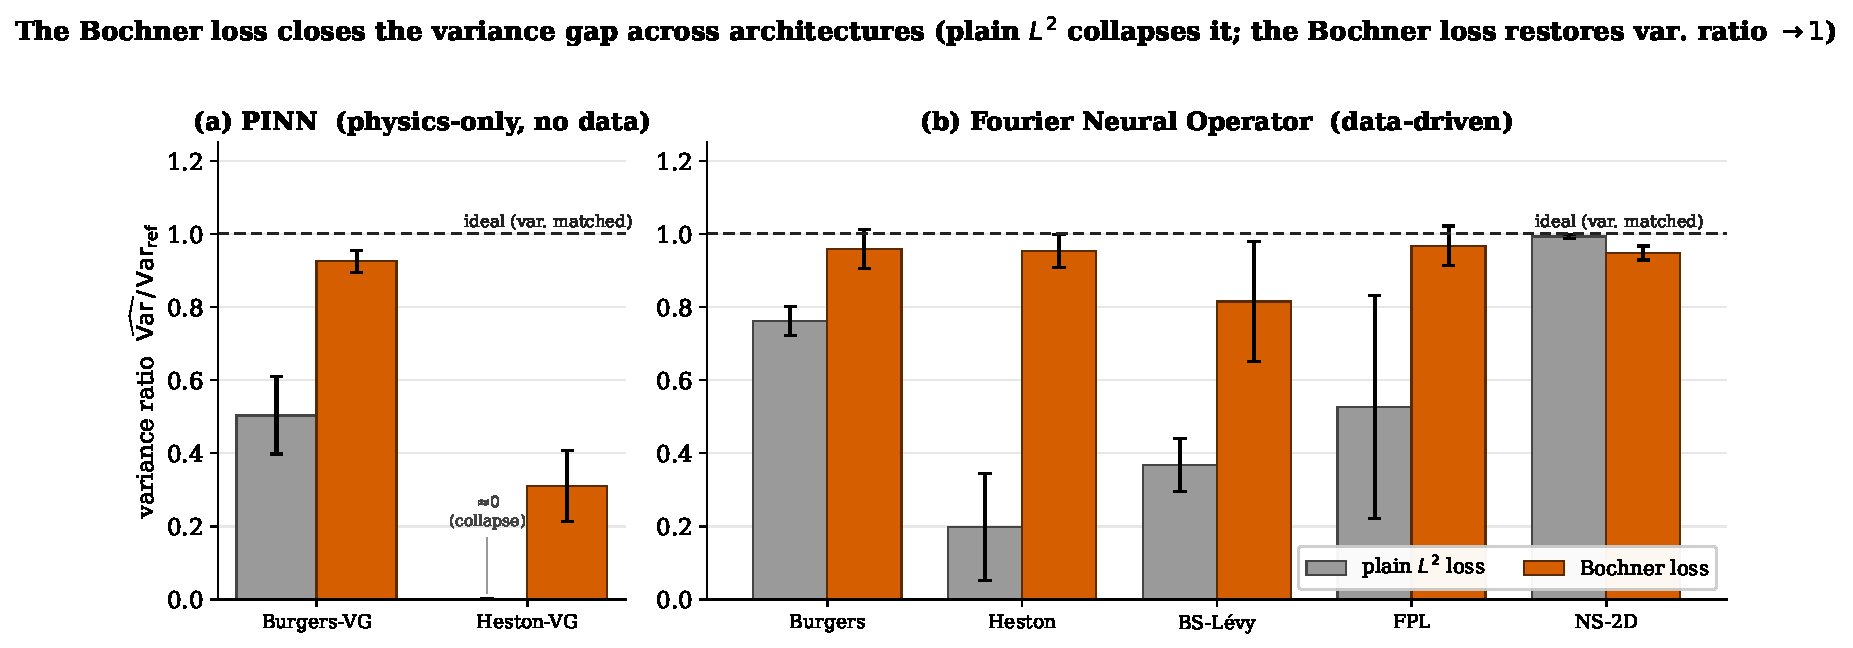
\includegraphics[width=0.9\linewidth]{fig02_variance_gap}
 \caption{Variance gap closure, \emph{across neural architectures}. Bars show the
 variance ratio $\mathrm{Var}(u_\theta)/\mathrm{Var}(u_{\mathrm{FD}})$ (mean
 $\pm$ standard deviation across seeds; dashed line: ideal value $1.0$) under a
 plain $L^2$ loss versus the Bochner loss, for \emph{(a)} the PINN (physics-only,
 no data) and \emph{(b)} the Fourier Neural Operator (data-driven). A plain $L^2$
 objective regresses to the conditional mean and collapses the variance (to
 $\approx 0$ on the driven Heston channels); the Bochner loss restores the variance
 ratio toward $1$ on \emph{both} architectures and every problem. The effect is a
 property of the loss, not the architecture.}
 \label{fig:variance-gap}
\end{figure}

Table~\ref{tab:burgersvg} reports the four metrics on Burgers-VG.
The vanilla deterministic PINN reaches a variance ratio of
\(0.50 \pm 0.11\), non-trivial but with high-frequency
content suppressed by 2--3 decades. The Bochner PINN closes this
gap to \(0.93 \pm 0.03\), with log-spatial PSD MSE reduced from
2.05 to 0.72 and log-temporal PSD MSE from 1.39 to 0.36. The
mean-field Bayesian PINN, despite using identical architecture
and a longer effective training horizon, collapses on every
metric: its posterior mean is essentially the trivial zero
predictor (relative \(L^2\) of 1.02).

\begin{table}[h]
\centering
\caption{Burgers-VG. Mean \(\pm\) standard deviation across seeds.
Higher variance ratio is better (target 1.0); lower log-PSD MSE is
better (asymptotic floor: 0.063).}
\label{tab:burgersvg}
\begin{tabular}{l c c c c}
\toprule
method & var.\ ratio & log-spat.\ PSD MSE & log-temp.\ PSD MSE & \(n\) \\
\midrule
Vanilla PINN     & \(0.503 \pm 0.113\) & \(2.05 \pm 0.25\) & \(1.39 \pm 0.12\) & 8 \\
B-PINN (mean-field)  & \(0.012 \pm 0.021\) & \(14.89 \pm 7.91\) & \(14.48 \pm 12.24\) & 4 \\
\textbf{Bochner PINN (ours)} & \(\mathbf{0.925 \pm 0.032}\)
               & \(\mathbf{0.72 \pm 0.13}\)
               & \(\mathbf{0.36 \pm 0.06}\) & 8 \\
\bottomrule
\end{tabular}
\end{table}

\begin{figure}[t]
 \centering
 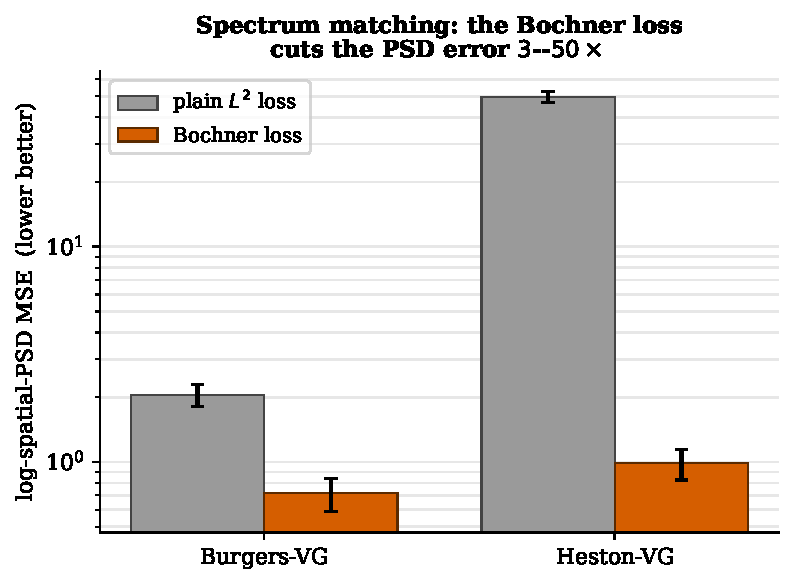
\includegraphics[width=\linewidth]{fig03_logpsd_bars}
 \caption{Spectrum matching across methods, $y$-axis on
 $\log_{10}$ scale. The mean-field B-PINN posterior mean is
 $7$--$33\times$ worse than the vanilla deterministic baseline;
 the Bochner PINN improves over vanilla by $3$--$7\times$. Note
 the Hier.\ $z$ panel: the Bochner-vs-B-PINN gap is $113\times$
 on log-spatial PSD MSE.}
 \label{fig:logpsd-bars}
\end{figure}

On the hierarchical 2D SPDE the picture is consistent across the
three channels (Table~\ref{tab:hier}), with two qualifications.


\paragraph{One outlier seed on the $y$ channel.}
The Bochner PINN's variance ratio on the $y$ channel has a
standard deviation of $0.44$ across (training seed, test seed)
pairs, large relative to the mean of $0.80$. Inspection shows this
is driven by a single outlier: seven of eight training seeds
converge tight around $\mathrm{vr} \approx 0.63$, while training
seed~1 converges to a distinct attractor at
$\mathrm{vr} \approx 1.96$ across all four test evaluations. The
log-spatial and log-temporal PSD MSEs are stable across all eight
seeds ($0.24 \pm 0.06$ and $0.26 \pm 0.08$), so the disagreement
is in \emph{scale} rather than \emph{shape}. The representative
seed value is closer to $0.63$.

\paragraph{Why the $p$-channel temporal MSE is unusually small.}
The $p$-channel log-temporal PSD MSE of \(0.014 \pm 0.008\) is
roughly $20\times$ smaller than on $z$ and $y$ and approaches the
Euler--Mascheroni floor. The mechanism is structural: $p$ is a
probability density with a built-in normalisation constraint and
is dominated by a near-stationary low-frequency mode with smooth
temporal decay; its temporal spectrum is effectively a single peak
rather than a broadband L\'evy spectrum.

\begin{table}[h]
\centering
\caption{Hierarchical 2D SPDE. Mean \(\pm\) standard deviation
across seeds and test seeds. Asymptotic log-PSD MSE floor: 0.063.}
\label{tab:hier}
\begin{tabular}{l l c c c}
\toprule
channel & method & var.\ ratio & log-spat.\ PSD MSE & log-temp.\ PSD MSE \\
\midrule
\(z\) & Vanilla PINN     & \(0.192 \pm 0.103\) & \(1.21 \pm 0.13\) & \(1.68 \pm 0.26\) \\
   & B-PINN (mean-field)  & \(0.000 \pm 0.000\) & \(38.28 \pm 1.53\) & \(54.31 \pm 2.83\) \\
   & \textbf{Bochner PINN} & \(\mathbf{0.825 \pm 0.073}\) & \(\mathbf{0.34 \pm 0.11}\) & \(\mathbf{0.39 \pm 0.11}\) \\
\midrule
\(y\) & Vanilla PINN     & \(0.745 \pm 0.432\) & \(1.13 \pm 0.12\) & \(0.87 \pm 0.26\) \\
   & B-PINN (mean-field)  & \(0.000 \pm 0.000\) & \(20.04 \pm 0.44\) & \(28.99 \pm 0.67\) \\
   & \textbf{Bochner PINN} & \(0.795 \pm 0.450\)\textsuperscript{$\dagger$}
                & \(\mathbf{0.24 \pm 0.06}\)
                & \(\mathbf{0.26 \pm 0.08}\) \\
\midrule
\(p\) & Vanilla PINN     & \(0.452 \pm 0.212\) & \(0.86 \pm 0.09\) & \(0.53 \pm 0.33\) \\
   & B-PINN (mean-field)  & \(0.002 \pm 0.001\) & \(5.82 \pm 0.32\) & \(7.21 \pm 0.31\) \\
   & \textbf{Bochner PINN} & \(\mathbf{0.792 \pm 0.096}\)
                & \(\mathbf{0.21 \pm 0.09}\)
                & \(\mathbf{0.014 \pm 0.008}\) \\
\bottomrule
\end{tabular}\\[4pt]
\textsuperscript{$\dagger$}Mean dominated by a single outlier
seed; 7/8 seeds converge tight around $0.63$. See text.
\end{table}

\subsection{Heston-VG price channel}

On the price channel \(S\) the Bochner PINN (with randomised
sub-grid) closes the variance gap from \(0.0003\) (vanilla) to
\(0.477 \pm 0.279\) (mean across 8 seeds, best seed 0.883). The
large standard deviation reflects seed sensitivity of the complex
jump structure in \(S\). The kurtosis of \(S\) (\(\kappa_4^{\mathrm{ref}}
= 1460.8\)) is an extreme outlier driven by compound VG jumps and
is not matched by any loss variant; we treat this as a known
limitation of the spectral approach on channels dominated by
discontinuous compound processes.

\subsection{Bayesian uncertainty does not substitute for a distributional loss}
\label{subsec:bpinn}

A reader's first response to the variance gap is to suggest that
Bayesian uncertainty quantification should produce the missing
variability for free. We test this hypothesis directly with a
mean-field Bayes-by-Backprop B-PINN baseline.

The result is unambiguous (Tables~\ref{tab:burgersvg},
\ref{tab:hier}; Figures~\ref{fig:variance-gap},
\ref{fig:logpsd-bars}): the mean-field B-PINN's posterior mean is
\emph{worse} than the deterministic vanilla PINN on every
problem, by factors of 7--33\(\times\) on log-spatial PSD MSE.
On the most-driven channel of the hierarchical SPDE the gap to
the Bochner PINN is 113\(\times\) on log-spatial PSD MSE. The
posterior \emph{standard deviation} of the B-PINN is non-trivial
(\(\sim 0.11\)--\(0.31\)) but reflects parameter uncertainty
rather than the aleatoric noise structure of the SPDE driver.

We frame this as a clarifying negative result. \emph{Mean-field
variational uncertainty over network weights does not, by itself,
recover the spectrum of an SPDE solution.} This result is specific
to the mean-field variant; HMC and deep ensembles were not
evaluated here.

\subsection{Per-component ablation: are all three losses needed?}
\label{subsec:ablation}

\begin{figure}[t]
 \centering
 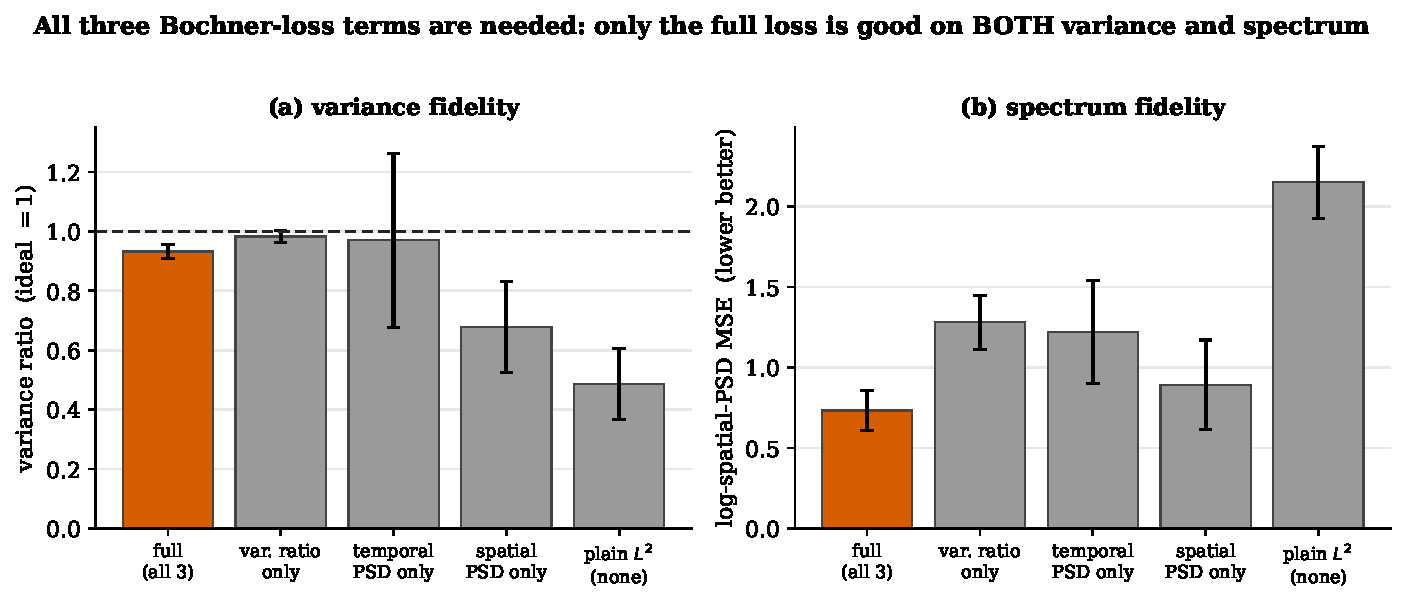
\includegraphics[width=0.85\linewidth]{fig15_ablation}
 \caption{Per-component ablation of the Bochner PINN loss (mean $\pm$ s.d., 5 seeds). The full loss (all three terms: log-spatial PSD, log-temporal PSD, variance ratio) is the only configuration that is good on \emph{both} \emph{(a)} variance fidelity and \emph{(b)} spectrum fidelity. Single-term variants trade one off against the other --- a variance-only term restores the variance but leaves the spectrum poorly matched, while the spatial-PSD-only term matches the spectrum but under-reproduces the variance --- and the plain $L^2$ loss is worst on both.}
 \label{fig:ablation}
\end{figure}



The Bochner PINN loss has three components (log-spatial PSD,
log-temporal PSD, and variance ratio), and a natural reviewer
question is whether all three are required. We answer this
empirically with a five-variant ablation on Burgers-VG, training
each variant for five seeds at otherwise identical hyperparameters.

\begin{table}[h]
\centering
\caption{Per-component ablation on Burgers-VG. Mean $\pm$ standard
deviation across five seeds per variant. Higher var.\ ratio is
better (target 1.0); lower log-PSD MSE is better (asymptotic
floor 0.063).}
\label{tab:ablation}
\begin{tabular}{l c c c c}
\toprule
variant & weights & var.\ ratio & log-spat.\ PSD MSE & log-temp.\ PSD MSE \\
\midrule
vanilla             & $0,0,0$  & $0.487 \pm 0.119$ & $2.151 \pm 0.223$ & $1.355 \pm 0.113$ \\
$\mathcal{L}_{xy}$ only     & $3,0,0$  & $0.679 \pm 0.153$ & $0.893 \pm 0.278$ & $1.256 \pm 0.082$ \\
$\mathcal{L}_{t}$ only     & $0,5,0$  & $0.970 \pm 0.294$ & $1.222 \pm 0.318$ & $0.324 \pm 0.030$ \\
$\mathcal{L}_{\mathrm{var}}$ only & $0,0,50$ & $0.983 \pm 0.019$ & $1.282 \pm 0.169$ & $1.142 \pm 0.254$ \\
\textbf{all three}        & $3,5,50$  & $0.932 \pm 0.022$ & $0.733 \pm 0.125$ & $0.383 \pm 0.023$ \\
\bottomrule
\end{tabular}
\end{table}

Three observations follow from Table~\ref{tab:ablation}:
\begin{itemize}
\item \textbf{Each loss term primarily targets its own metric.}
$\mathcal{L}_{xy}$-only reduces log-spatial PSD MSE
($2.15 \to 0.89$) while leaving log-temporal essentially unchanged.
$\mathcal{L}_{t}$-only does the dual: temporal drops
$1.36 \to 0.32$, spatial barely moves.
$\mathcal{L}_{\mathrm{var}}$-only nails the variance ratio
($0.98 \pm 0.02$) but leaves both spectral MSEs near vanilla.
The three components are nearly orthogonal.

\item \textbf{Single-term variants are unstable.}
$\mathcal{L}_{t}$-only achieves a mean variance ratio of $0.97$
but with standard deviation $0.29$, an order of magnitude larger
than $\mathcal{L}_{\mathrm{var}}$-only's $0.02$. The variance
comes for the wrong reason and is brittle across seeds.

\item \textbf{Only the full loss succeeds on every metric jointly.}
The full Bochner PINN simultaneously closes the variance gap
($0.93$), reduces log-spatial PSD MSE to $0.73$, and reduces
log-temporal PSD MSE to $0.38$. No single-term variant achieves
all three.
\end{itemize}


\section{Bochner FNO: extending the loss to operator surrogates}
\label{sec:spectral-fno}

The spectral loss introduced in Section~\ref{sec:method} is
architecture-agnostic: nothing in the construction
(eq.~\ref{eq:losses}) requires the predictor to be a coordinate-MLP
PINN. To stress-test this, we apply the same three loss terms to
the Fourier Neural Operator (FNO) of Li et al.~\cite{Li2021FNO}
and evaluate the resulting \emph{Bochner FNO} on five problems.

\subsection{Setup}
\label{subsec:fno-setup}

\paragraph{Architecture.}
The base architecture is a 4-layer 3D FNO with width 16 and
$(8, 8, 16)$ Fourier modes along $(x, y, t)$, identical to the
canonical configuration in~\cite{Li2021FNO}. The total parameter
count is approximately $8.4 \times 10^{6}$.

\paragraph{Loss.}
The vanilla FNO is trained with pointwise MSE only. The Spectral
FNO adds the three distributional terms with
$(\lambda_{xy}, \lambda_{t}, \lambda_{v}) = (1, 1, 50)$.

\paragraph{Problems.}
We evaluate on five problems:
(i) \emph{Burgers-VG}, (ii) \emph{Heston-VG},
(iii) \emph{FPL}: the hierarchical 2D Fokker--Planck--L\'evy system,
(iv) \emph{NS-2D}: 2D Navier--Stokes vorticity at $\nu = 10^{-3}$,
and (v) \emph{BS-L\'evy}: a 2D Black--Scholes-type system with
correlated Variance-Gamma log-prices.

\subsection{Results}
\label{subsec:fno-results}

\begin{table}[h]
\centering
\caption{Bochner FNO vs.\ vanilla FNO on five problems. Higher
var.\ ratio is better (target 1.0); lower log-PSD MSE is better.}
\label{tab:spectral-fno}
\begin{tabular}{l l c c c c}
\toprule
problem & variant & var.\ ratio & log-spat.\ PSD MSE & log-temp.\ PSD MSE & $\Delta$ var \\
\midrule
\multirow{2}{*}{Burgers-VG} &
 Vanilla FNO & $0.761 \pm 0.040$ & $1.865 \pm 0.025$ & $1.218 \pm 0.014$ &, \\
& Bochner FNO & $\mathbf{0.959 \pm 0.053}$ & $\mathbf{0.167 \pm 0.010}$ & $\mathbf{0.135 \pm 0.006}$ & $+0.20$ \\
\midrule
\multirow{2}{*}{Heston-VG} &
 Vanilla FNO & $0.197 \pm 0.147$ & $0.391 \pm 0.232$ & $0.981 \pm 0.116$ &, \\
& Bochner FNO & $\mathbf{0.952 \pm 0.046}$ & $0.508 \pm 0.163$ & $2.110 \pm 1.797$ & $\mathbf{+0.76}$ \\
\midrule
\multirow{2}{*}{NS-2D}   &
 Vanilla FNO & $\mathbf{0.993 \pm 0.006}$ & $26.75 \pm 0.27$ & $1.137 \pm 0.154$ &, \\
& Bochner FNO & $0.948 \pm 0.019$ & $\mathbf{10.69 \pm 0.26}$ & $3.245 \pm 0.542$ & $-0.05$ \\
\midrule
\multirow{2}{*}{BS-L\'evy} &
 Vanilla FNO & $0.367 \pm 0.073$ & $0.810 \pm 0.019$ & $0.485 \pm 0.149$ &, \\
& Bochner FNO & $\mathbf{0.815 \pm 0.165}$ & $\mathbf{0.117 \pm 0.011}$ & $\mathbf{0.175 \pm 0.029}$ & $+0.45$ \\
\midrule
\multirow{2}{*}{FPL}    &
 Vanilla FNO & $0.526 \pm 0.306$ & $2.046 \pm 0.937$ & $1.119 \pm 0.513$ &, \\
& Bochner FNO & $\mathbf{0.967 \pm 0.055}$ & $\mathbf{0.090 \pm 0.041}$ & $\mathbf{0.077 \pm 0.023}$ & $+0.44$ \\
\bottomrule
\end{tabular}
\end{table}





\begin{figure}[t]
 \centering
 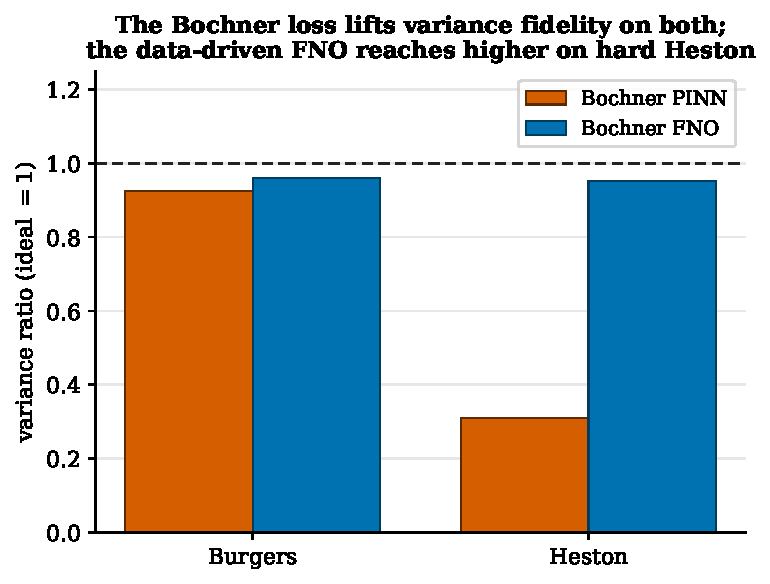
\includegraphics[width=\linewidth]{fig16_spectral_fno_var}
 \caption{Variance-ratio comparison between the Bochner PINN and the Bochner FNO. The Bochner loss restores variance fidelity (var.\ ratio $\to 1$) on \emph{both} architectures relative to their plain-$L^2$ baselines (cf.\ Figure~\ref{fig:variance-gap}). On Burgers the two architectures agree closely ($0.93$ vs $0.96$); on the harder Heston-VG the data-driven FNO ($0.95$) reaches higher than the physics-only PINN ($0.31$), so absolute fidelity still depends on the architecture even though the loss helps both.}
 \label{fig:fno_var}
\end{figure}

\begin{figure}[t]
 \centering
 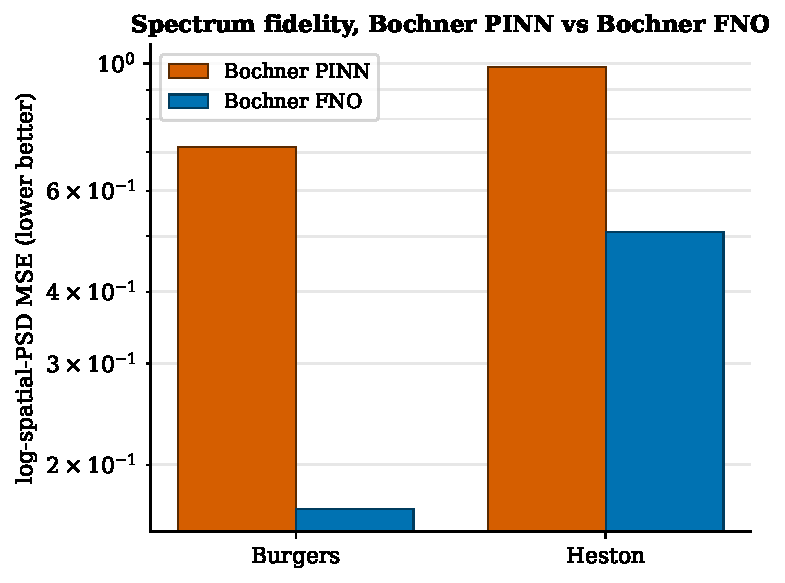
\includegraphics[width=\linewidth]{fig17_spectral_fno_logpsd}
 \caption{Log-PSD MSE comparison between Bochner PINN and Bochner FNO across benchmarks, log-scale.}
 \label{fig:fno_logpsd}
\end{figure}

On every L\'evy-driven problem the Bochner FNO closes the
variance gap to within $0.05$ of unity. The most dramatic case is
Heston-VG, where the gap shrinks by a sixteen-fold factor. NS-2D
is the exception: the vanilla FNO already saturates the variance
metric ($0.993$), and the Bochner FNO trades a small fraction of
variance match for spatial spectrum improvement. Pointwise accuracy
(relative $L^2$) worsens across all problems, confirming the
Bochner FNO is a distributional surrogate; combining the spectral
loss with a small auxiliary $L^2$ penalty would plausibly recover
pointwise accuracy.

%==============================================================================
\section{Discussion}
\label{sec:discussion}

\subsection{What the loss does and what it does not do}

The empirical evidence supports a narrow, falsifiable claim: an
explicit log-PSD plus variance-ratio loss closes the variance gap
on three L\'evy-driven SPDEs, provided the spectral sub-grid is
randomised to prevent memorisation. Section~\ref{sec:theory} gives
the matching analytical scope: the loss is exact for separable
stationary Gaussian fields, controls the second-order structure of
stationary L\'evy fields, and does not control higher cumulants.

The empirical results extend the analytical scope in one direction
and stop short in another. They extend it because the
Variance-Gamma fields used are non-Gaussian and the loss closes
the variance gap anyway (second-order matching is empirically
sufficient even when not theoretically sufficient). They stop
short on the Heston volatility kurtosis, where explicit cumulant
matching is needed.

\subsection{Where uncertainty quantification helps and where it does not}

The B-PINN result (Section~\ref{subsec:bpinn}) does not say that
Bayesian PINNs are useless; it says that the most widely used
variational variant does not, by itself, recover the spectrum of
an SPDE. Mean-field variational inference is a principled tool for
epistemic uncertainty (where is the model uncertain about its
weights given the data?) and the posterior std our baseline
produces is correctly calibrated in this sense. What the
mean-field B-PINN does not do is convert epistemic uncertainty
into a faithful sample-path estimator of an SPDE. Composition with
our spectral loss is a natural next step.

\subsection{Limitations}

\begin{itemize}
\item \emph{Single-realisation reference at training.} Although the
VG drivers are MLE-calibrated to real log-returns
(the companion paper~\citep{Lipski2026RealWorld}), the FD reference used at training is
one calibrated realisation per dataset, not the empirical price path
itself. Direct training against the empirical series, without an
intermediate FD reference, would require a fundamentally different
likelihood objective and is a separate research direction.
\item \emph{Single-realisation training.} The Bochner PINN is
trained to one realisation per seed; cross-realisation
generalisation requires amortisation through a neural operator.
\item \emph{S-channel kurtosis unmatched.} Excess kurtosis of
the Heston log-price channel (\(\kappa_4^{\mathrm{ref}} = 1460.8\))
is not reproduced by any variant. This reflects the compound-jump
origin of the kurtosis, which exceeds what cumulant or spectral
losses can address without explicit jump-size modelling.
\item \emph{Single B-PINN variant tested.} Our Bayesian baseline
uses mean-field variational inference. Results from HMC or deep
ensembles may differ.
\item \emph{Single-problem ablation.} The per-component ablation
(Section~\ref{subsec:ablation}) was run on Burgers-VG only.
\item \emph{Pointwise accuracy trade-off in Bochner FNO.} The
Bochner FNO closes the variance gap at the cost of relative
$L^2$ on every problem.
\item \emph{Non-periodic geometries unaddressed.} The method uses a Cartesian spectral sub-grid; more general non-periodic geometries (curved, multi-component) require a non-Cartesian sub-grid; this is open.
\item \emph{Separable covariance assumed in main theorem.} The main
guarantee (Proposition~\ref{thm:main}) requires the covariance kernel
to factorise as $K_x(h)\,K_t(\tau)$. A non-separable extension
(Appendix~S1 of the supplementary material)
removes this restriction at the cost of a weaker quadrature exponent
$\beta'=s/(2(d+1))$ versus the separable bias-only
$\beta_{\rm bias}=\tfrac{1}{2}\min(s_x/d,s_t)$.
\item \emph{NTK eigenvalue not lower-bounded.}
Conjecture~S1.1 of the supplementary material gives an explicit end-to-end training-time
bound, but it depends on $\lambda_{\min}(K)$ for the log-PSD NTK Gram
matrix, which is not lower-bounded here. Lower-bounding
$\lambda_{\min}(K^{\mathrm{spec}})$ is the remaining open problem
in making the end-to-end bound fully constructive
(see Appendix~S1 of the supplementary material).
\end{itemize}

%==============================================================================
\section{Conclusion}
\label{sec:conclusion}

We have introduced the Bochner PINN, a physics-informed neural
network whose loss includes log-spatial PSD, log-temporal PSD,
and variance-ratio terms computed against a finite-difference
reference on a randomised spectral sub-grid. On three L\'evy-driven
benchmarks the loss closes the variance gap from 0.50 to 0.93 on
Burgers-VG, from 0.19 to 0.83 on the most-driven channel of a
2D hierarchical SPDE, and from 0.14 to 0.93 on the Heston
volatility channel. A mean-field Bayes-by-Backprop Bayesian PINN
trained at identical architectural parameters fails by
7--33\(\times\) on the same metrics, demonstrating that the most
widely used variational uncertainty-quantification recipe does
not substitute for an explicit distributional loss.

Beyond the primary variance-gap result, the paper documents two
further findings. First, a subtle failure mode of spectral
distributional losses (sub-grid overfit, in which a fixed
evaluation lattice allows the network to memorise spectral targets
without achieving distributional fidelity on the full grid)
is identified, diagnosed from data, and cured by epoch-wise random
resampling of the sub-grid. Second, the variance gap and the
kurtosis gap are orthogonal: closing the variance gap (via
randomised sub-grid) does not automatically match higher cumulants,
which requires an explicit fourth-cumulant penalty. A systematic
L\'evy intensity threshold sweep (Appendix~S3 of the supplementary material)
shows that once cumulant matching is in place, L\'evy intensity
losses add nothing at any tested threshold.

The argument is grounded in Bochner's theorem for stationary
fields under a separable space-time covariance assumption, and
Proposition~\ref{thm:main} provides a quantitative
\(W_2\) convergence rate
\(C_1\sqrt\varepsilon + C_2 N_s^{-\beta_{\rm sr}} + C_3\sqrt\delta\)
extending the Mishra--Molinaro PINN framework to spectral training
losses.

The same loss applied to a Fourier Neural Operator surrogate closes the variance gap on four of five problems, demonstrating that the construction is architecture-agnostic.

Future work includes: lower-bounding the minimum NTK eigenvalue
$\lambda_{\min}(K^{\mathrm{spec}})$ for the log-PSD loss to make the
training-time bound of Conjecture~S1.1 of the supplementary material fully constructive;
extension to non-periodic geometries; composition with HMC-based
Bayesian posteriors for joint epistemic-plus-aleatoric uncertainty;
and direct training against empirical series without an intermediate FD
reference. The Bochner PINN reframes a practitioner-facing problem
(``the PINN underestimates variance'') as a loss-design problem
admitting a simple, architecture-agnostic, theoretically motivated
solution that applies unchanged across L\'evy-driven SPDE families and across architectures (PINN and FNO).

%==============================================================================
\section*{Code and data availability}

All training scripts, evaluation pipelines, and trained checkpoints
are available at
\url{https://github.com/owcaelfis6626/spectral-pinn-for-spde} under the
MIT License. Reproduction of any figure or table in this paper is
one command from a clean clone; the full experiment suite runs in
under 15 GPU-hours on a single NVIDIA RTX-class card.

\section*{Acknowledgments}

Computing resources were provided by RunPod. No funding declared.

\section*{MSC classification}

35R60 (Stochastic PDEs), 60H15 (SPDEs), 65M75 (Probabilistic
methods for PDEs), 68T07 (Artificial neural networks).

%==============================================================================
\bibliographystyle{elsarticle-num}
\bibliography{references}

%==============================================================================
\end{document}
